\medskip

La directrice d'une école souhaite réaliser une étude auprès des étudiants qui ont passé l'examen de fin d'étude, pour analyser la façon dont ils pensent avoir réussi cet examen.

\smallskip

Pour cette étude, on demande aux étudiants à l'issue de l'examen de répondre individuellement à la question : \og Pensez-vous avoir réussi l'examen ?\fg.

\smallskip

Seules les réponses  \og oui\fg{} ou \og non \fg{} sont possibles, et on observe que $91,7\,\%$ des étudiants interrogés ont répondu \og oui\fg.

Suite à la publication des résultats à l'examen, on découvre que :
\begin{itemize}
	\item $65\,\%$ des étudiants ayant échoué ont répondu \og non\fg{} ;
	\item $98\,\%$ des étudiants ayant réussi ont répondu \og oui\fg.
\end{itemize}

On interroge au hasard un étudiant qui a passé l'examen.

On note $R$ l'évènement \og l'étudiant a réussi l'examen \fg{} et $Q$ l'évènement \og l'étudiant a répondu \og oui\fg{}  à la question\fg{}.

Pour un évènement $A$ quelconque, on note $P(A)$ sa probabilité et $\overline{A}$ son évènement contraire.

\medskip

\textbf{Dans tout l'exercice, les probabilités sont, si besoin, arrondies à \boldmath$10^{-3}$\unboldmath{} près.}
\begin{enumerate}
	\item Préciser les valeurs des probabilités $P(Q)$ et $P_{\overline{R}}\left(\overline{Q}\right)$.

	\item On note $x$ la probabilité que l'étudiant interrogé ait réussi l'examen.
	\begin{enumerate}
		\item Recopier et compléter l'arbre pondéré ci-dessous.

		\begin{center}
			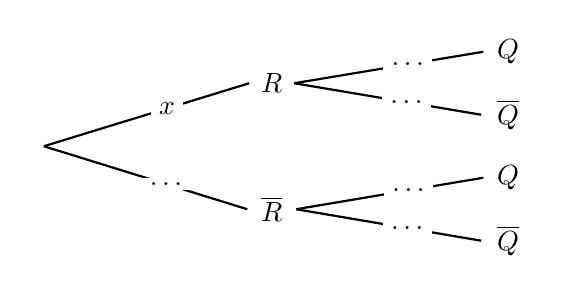
\begin{tikzpicture}[xscale=1,yscale=1,baseline={(R.base)}]
				
				\tikzstyle{fleche}=[-,>=latex,thick]
				\tikzstyle{noeud}=[fill=white,circle,inner sep=2pt]
				\tikzstyle{feuille}=[fill=white,circle,inner sep=2pt]
				\tikzstyle{etiquette}=[pos=0.6,fill=white, inner xsep=3pt, inner ysep=1.5pt]
				
				\def\DistanceInterNiveaux{3}
				\def\DistanceInterFeuilles{0.8}
				
				\def\NiveauA{(0)*\DistanceInterNiveaux}
				\def\NiveauB{(1)*\DistanceInterNiveaux}
				\def\NiveauC{(2)*\DistanceInterNiveaux}
				\def\InterFeuilles{(-1)*\DistanceInterFeuilles}
				
				\node[noeud] (R) at ({\NiveauA},{(1.5)*\InterFeuilles}) {};
				\node[noeud] (Ra) at ({\NiveauB},{(0.5)*\InterFeuilles}) {$R$};
				\node[feuille] (Raa) at ({\NiveauC},{(0)*\InterFeuilles}) {$Q$};
				\node[feuille] (Rab) at ({\NiveauC},{(1)*\InterFeuilles}) {$\overline{Q}$};
				\node[noeud] (Rb) at ({\NiveauB},{(2.5)*\InterFeuilles}) {$\overline{R}$};
				\node[feuille] (Rba) at ({\NiveauC},{(2)*\InterFeuilles}) {$Q$};
				\node[feuille] (Rbb) at ({\NiveauC},{(3)*\InterFeuilles}) {$\overline{Q}$};
				
				\draw[fleche] (R.east)--(Ra.west)node[etiquette] {$x$};
				\draw[fleche] (Ra.east)--(Raa.west) node[etiquette] {$\ldots $};
				\draw[fleche] (Ra.east)--(Rab.west) node[etiquette] {$\ldots $};
				\draw[fleche] (R.east)--(Rb.west) node[etiquette] {$\ldots $};
				\draw[fleche] (Rb.east)--(Rba.west) node[etiquette] {$\ldots $};
				\draw[fleche] (Rb.east)--(Rbb.west) node[etiquette] {$\ldots $};
			\end{tikzpicture}
		\end{center}

		\item  Montrer que $x=0,9$.
	\end{enumerate}

	\item L'étudiant interrogé a répondu \og oui\fg{}  à la question.
	
Quelle est la probabilité qu'il ait réussi l'examen?

	\item La note obtenue par un étudiant interrogé au hasard est un nombre entier entre 0 et 20 . On suppose qu'elle est modélisée par une variable aléatoire $N$ qui suit la loi binomiale de paramètres $(20 ~;~0,615)$.
	
	La directrice souhaite attribuer une récompense aux étudiants ayant
obtenu les meilleurs résultats.

À partir de quelle note doit-elle attribuer les récompenses pour que $65\,\%$ des étudiants soient récompensés?

	\item On interroge au hasard dix étudiants.
	
Les variables aléatoires $N_{1}, N_{2}, \ldots, N_{10}$ modélisent la note sur 20 obtenue à l'examen par chacun d'entre eux. On admet que ces variables sont indépendantes et suivent la même loi binomiale de paramètres $(20 ~;~ 0,615)$.\\
	Soit $S$ la variable définie par $S=N_{1}+N_{2}+\cdots+N_{10}$.\\
	Calculer l'espérance $E(S)$ et la variance $V(S)$ de la variable aléatoire $S$.


	\item On considère la variable aléatoire $M=\dfrac{S}{10}$.
	\begin{enumerate}
		\item Que modélise cette variable aléatoire $M$ dans le contexte de l'exercice ?
		\item Justifier que $E(M)=12,3$ et $V(M)=\np{0,47355}$.
		\item À l'aide de l'inégalité de Bienaymé-Tchebychev, justifier l'affirmation ci-dessous.

\smallskip

\og La probabilité que la moyenne des notes de dix étudiants pris au hasard soit strictement comprise entre 10,3 et 14,3 est d'au moins $80\,\%$ \fg.
	\end{enumerate}
\end{enumerate}

\medskip
